\documentclass{article}
\usepackage{amsmath}
\usepackage{graphicx}
\usepackage{subcaption}
\usepackage{polski}
\usepackage[utf8]{inputenc}


\begin{document}
\title{Sprawdzenie podstawowych własności ferroelektrycznych zachodzących w krysztale TGS.}
\date{}
\author{K.Dziubak, E.Klajmon\\Institute of Physics, Wrocław University of Technology, \\Wybrzeże
Wyspiańskiego 27, 50-370 Wrocław, Poland}
\maketitle
\pagenumbering{arabic}

W tym artykule przedstawione zostały układy pomiarowe, sposoby wykonywania oraz wyniki pomiarów, które miały na celu zbadanie podstawowych własności i zjawisk w materiałach ferroelektrycznych, t.j. polaryzacja spontaniczna, dwójłomność spontaniczna oraz przenikalność elektryczna.

\paragraph{}
\textbf{Słowa kluczowe}: dielektryk, ferroelektryk, polaryzacja spontaniczna, dwójłomność spontaniczna, przenikalność elektryczna.

\section{Wstęp}
\subsection{Podział dielektryków}
\begin{figure}[!h]
	\centering
	\includegraphics[width=0.7\linewidth]{podzial.png}
	\caption{Podział dielektryków.}
	\label{fig:podzial}
\end{figure}

Ferroelektryki, do których zalicza się badany przez nas kryształ TGS, są podgrupą dielektryków. \textbf{Dielektrykami} nazywamy materiały bardzo słabo przewodzące prąd elektryczny, w których występuje zjawisko polaryzacji dielektrycznej, czyli zjawisko utworzenia dipoli elektrycznych lub orientacji już istniejących dipoli w reakcji na przyłożone pole elektryczne. Podgrupą dielektryków są \textbf{piezoelektryki}, w których pod wpływem zewnętrznych naprężeń, na powierzchni materiału pojawiają się ładunki elektryczne. Podgrupą piezoelektryków są \textbf{piroelektryki}, które pod wpływem gradientu temperatury są w stanie generować siłę elektromotoryczną (SEM). Piroelektrykami nazywane są również kryształy o biegunowych osiach symetrii, tylko w nich może występować polaryzacja spontaniczna\cite{krajewski}. Podgrupą piroelektryków są \textbf{ferroelektryki}, których niektóre właściwości staramy się przybliżyć w tym artykule. Cały podział można zobaczyć na Rys.\ref{fig:podzial}.
\subsection{Podstawowe właściwości ferroelektryków}
Ferroelektryki są materiałami w których można zaobserwować zjawisko histerezy w zewnętrznym polu elektrycznym\cite{histereza}. \textbf{Histereza} jest zjawiskiem zależności aktualnego stanu układu od stanów w poprzedzających chwilach, czyli inaczej jest to opóźnienie w reakcji na czynnik zewnętrzny. Charakterystyczna dla wszystkich ferroelektryków jest \textbf{pętla histerezy} dielektrycznej pokazana na Rys.\ref{fig:histereza}.

\begin{figure}[!h]
	\centering
	\includegraphics[scale=0.3]{histereza.png}
	\caption{Przykładowa pętla histerezy zaobserwowana podczas badania zjawiska polaryzacji spontanicznej w krysztale TGS.}
	\label{fig:histereza}
\end{figure}

Ferroelektryki są dielektrykami nieliniowymi, co oznacza, że ich polaryzacja zależy od zewnętrznego pola elektrycznego w sposób nieliniowy. Dodatkowo w ferroelektrykach, dzięki temu że są również piroelektrykami, występuje polaryzacja nawet pod nieobecność zewnętrznego pola elektrycznego. Polaryzację tą nazywamy \textbf{polaryzacją spontaniczną}, a jej kierunek w ferroelektrykach możemy zmienić za pomocą zewnętrznego pola elektrycznego. Kolejną cechą tych materiałów jest \textbf{znakomita przenikalność elektryczna}, która najczęściej rośnie wraz z temperaturą materiału, aż do temperatury krytycznej, zwanej \textbf{temperaturą Curie}, powyżej której w ferroelektryku zanika polaryzacja spontaniczna, przenikalność zaczyna stopniowo spadać zgodnie z \textbf{prawem Curie-Weissa}\cite{krajewski}, a ferroelektryk gwałtownie traci swoje właściwości i staje się paraelektrykiem. Zjawisko to wynika ze zmiany fazy ciała stałego.
\subsection{Dwójłomność w ferroelektrykach}
Załóżmy wiązkę światła wychodzącą z polaryzatora. Posiada ona tylko wektory elektryczne, których kierunek jest zgodny z kierunkiem polaryzacji. Taką wiązkę nazywamy \textbf{spolaryzowaną}. Gdy przejdzie ona przez drugi polaryzator, nazywany analizatorem, jej natężenie $I$ jest zwykle mniejsze od natężenia światła $I_{0}$  padającego na analizator i zależy od kąta $\alpha$ między kierunkami polaryzacji obu przyrządów. Mówi o tym zależność odkryta przez francuskiego fizyka Étienne-Louis Malusa, dziś nazywana \textbf{prawem Malusa}: \cite{malus}
\begin{equation}
I=I_{0}cos^{2}\alpha
\end{equation}
Spolaryzowana wiązka światła padając na kryształ ulega rozdzieleniu na dwie wzajemnie prostopadłe spolaryzowane wiązki - promień zwyczajny i promień nadzwyczajny - poruszające się z różnymi prędkościami. To zjawisko nazywamy \textbf{dwójłomnością}. Miarą dwójłomności jest różnica współczynników załamania promienia nadzwyczajnego i zwyczajnego\cite{dwoj}:
\begin{equation}
\Delta n = n_{e} - n_{o}
\end{equation}
W kryształach \textbf{anizotropowych}, czyli takich w których właściwości fizyczne zależą od kierunku, możemy być świadkami zjawiska nazywanego \textbf{dwójłomnością spontaniczną}, gdzie zjawisko to występuje naturalnie. Zjawisko to polega na zmianie miary dwójłomności $\delta(\Delta n)$ w zależności od temperatury. Spolaryzowana wiązka światła padając na kryształ ulega rozdzieleniu na wzajemnie prostopadle spolaryzowane wiązki poruszające się z różnymi prędkościami. Po wyjściu z kryształu następuje interferencja obu promieni, a jej wynikiem w zależności od różnicy faz jest wiązka spolaryzowana liniowo, kołowo lub eliptycznie. Różnica faz w obu wiązkach spowodowana jest różnica drogi przebytej w krysztale. Dla kryształu TGS, który jest centrosymetryczny w fazie paraelektrycznej anomalna część dwójłomności spontanicznej obserwowanej w fazie ferroelektrycznej, ma charakter spontanicznego efektu Kerra opisywanego równaniem $\delta \Gamma = r\cdot P_{s}^{2}$, gdzie r to współczynnik elektrooptyczny, a $P_{s}$ to polaryzacja spontaniczna.

\section{Układy pomiarowe}
\subsection{Polaryzacja spontaniczna}

\begin{figure}[!h]
	\centering
 	\includegraphics[width=0.7\linewidth]{setup1.png}
 	\caption{Schemat zestawu pomiarowego do badania polaryzacji spontanicznej.}
 	\label{fig:setup1}
\end{figure}

Układ którego użyliśmy do pomiaru polaryzacji spontanicznej i pola koercji pokazany jest na Rys.\ref{fig:setup1}. Jego głównym elementem jest odizolowana termicznie komora pomiarowa, w której znajdował się kryształ TGS. Temperaturę w komorze termicznej regulowaliśmy za pomocą \textit{UNIPAN Temperature Controller 660}, a bieżącą jej wartość monitorowaliśmy za pomocą układu termopary. Do zapewnienia prawidłowej pracy termopary użyliśmy miernika METEX ustawionego na zakres miliwoltów oraz mieszaniny lodu z wodą w osobnym termosie. Całość była podłączona do mostka DDP (Diamanta–Drencka–Pepinskiego), którego pracę na bieżąco wyświetlał oscyloskop.

\subsection{Przenikalność elektryczna}

\begin{figure}[!h]
	\centering
	\includegraphics[width=0.8\linewidth]{setup3.png}
	\caption{Schemat zestawu pomiarowego do badania przenikalności elektrycznej.}
	\label{fig:setup3}
\end{figure}

Przenikalność elektryczną zbadaliśmy dzięki układowi pokazanemu na Rys.\ref{fig:setup3}. W termostacie znajduje się kondensator wykonany z kryształu TGS, do którego podłączony jest mostek objętościowy Escort ELC-3133A. Całość podłączona jest do regulatora temperatury \textit{UNIPAN Temperature Controller 660}, a temperatura wewnątrz termostatu monitorowana jest za pomocą termopary. Do prawidłowego działania układu termopary potrzebny jest termos z mieszaniną lodu i wody (o temperaturze zbliżonej do $0^{o}C$) i miernik METEX, używany jako miliwoltomierz. Całość podłączona jest do komputera, a program $Escort$ odczytując bieżące parametry pojemności kondensatora dla danej temperatury, rysuje aktualny wykres oraz zapisuje wyniki.

\subsection{Dwójłomność spontaniczna}

\begin{figure}[!h]
	\centering
	\includegraphics[width=0.7\linewidth]{setup2.png}
	\caption{Schemat zestawu pomiarowego do badania dwójłomności spontanicznej.}
	\label{fig:setup2}
\end{figure}

Podczas badania zjawiska dwójłomności spontanicznej posłużyliśmy się zestawem pokazanym na Rys.\ref{fig:setup2}. Jego główną częścią był termostat z kryształem TGS w środku. Jego temperatura była kontrolowana przez \textit{UNIPAN Temperature Controller 660}, a monitorowana - tak samo jak w przypadku badania polaryzacji spontanicznej - przez miernik METEX. Przed i za termostatem ustawione zostały dwa polaryzatory, nazwane kolejno polaryzatorem i analizatorem. Za analizatorem znajdowała się fotokomórka oraz podłączony do niej mikroamperomierz. Obydwa mierniki były podłączone do komputera, który za pomocą odpowiedniego programu sczytywał dane, robił z nich wykres, a następnie zapisywał wyniki wartości natężenia światła w zależności od temperatury.

\section{Pomiary i wyniki}
\subsection{Polaryzacja spontaniczna}

Badanie polaryzacji spontanicznej odbywało się poprzez odczyt i zapis pętli histerezy wyświetlanych na oscyloskopie, w trakcie zmieniania temperatury próbki. Najpierw ogrzewaliśmy próbkę od temperatury pokojowej, aż do temperatury w której zaobserwowaliśmy kompletny zanik pętli histerezy. Była to w naszym przypadku temperatura około $50^{o}C$. Następnie wyciągnęliśmy próbkę i w procesie swobodnego chłodzenia powtórzyliśmy badanie, aż do uzyskania temperatury około $34^{o}C$, ponieważ w okolicach tej temperatury swobodne chłodzenie próbki przebiegało już bardzo wolno. Warto wspomnieć, że do wysycenia pętli wystarczyło napięcie $194V$, a nasza próbka miała grubość $1,6\cdot10^{-3}m$. Podstawiając te wartości do wzoru:

\begin{equation}
E_{max}=\dfrac{U_{max}}{d}=\dfrac{\sqrt{2 \cdot U_{sk}}}{d}
\end{equation}

obliczyliśmy maksymalne pole elektryczne przyłożone do próbki. Wynosiło ono $1,21\cdot 10^{5} \dfrac{V}{m^{2}}$. Przykładowe pętle histerezy zaobserwowane podczas ogrzewania próbki widoczne na Rys.\ref{fig:Graph31}.

\begin{figure}[!h]
	\centering
	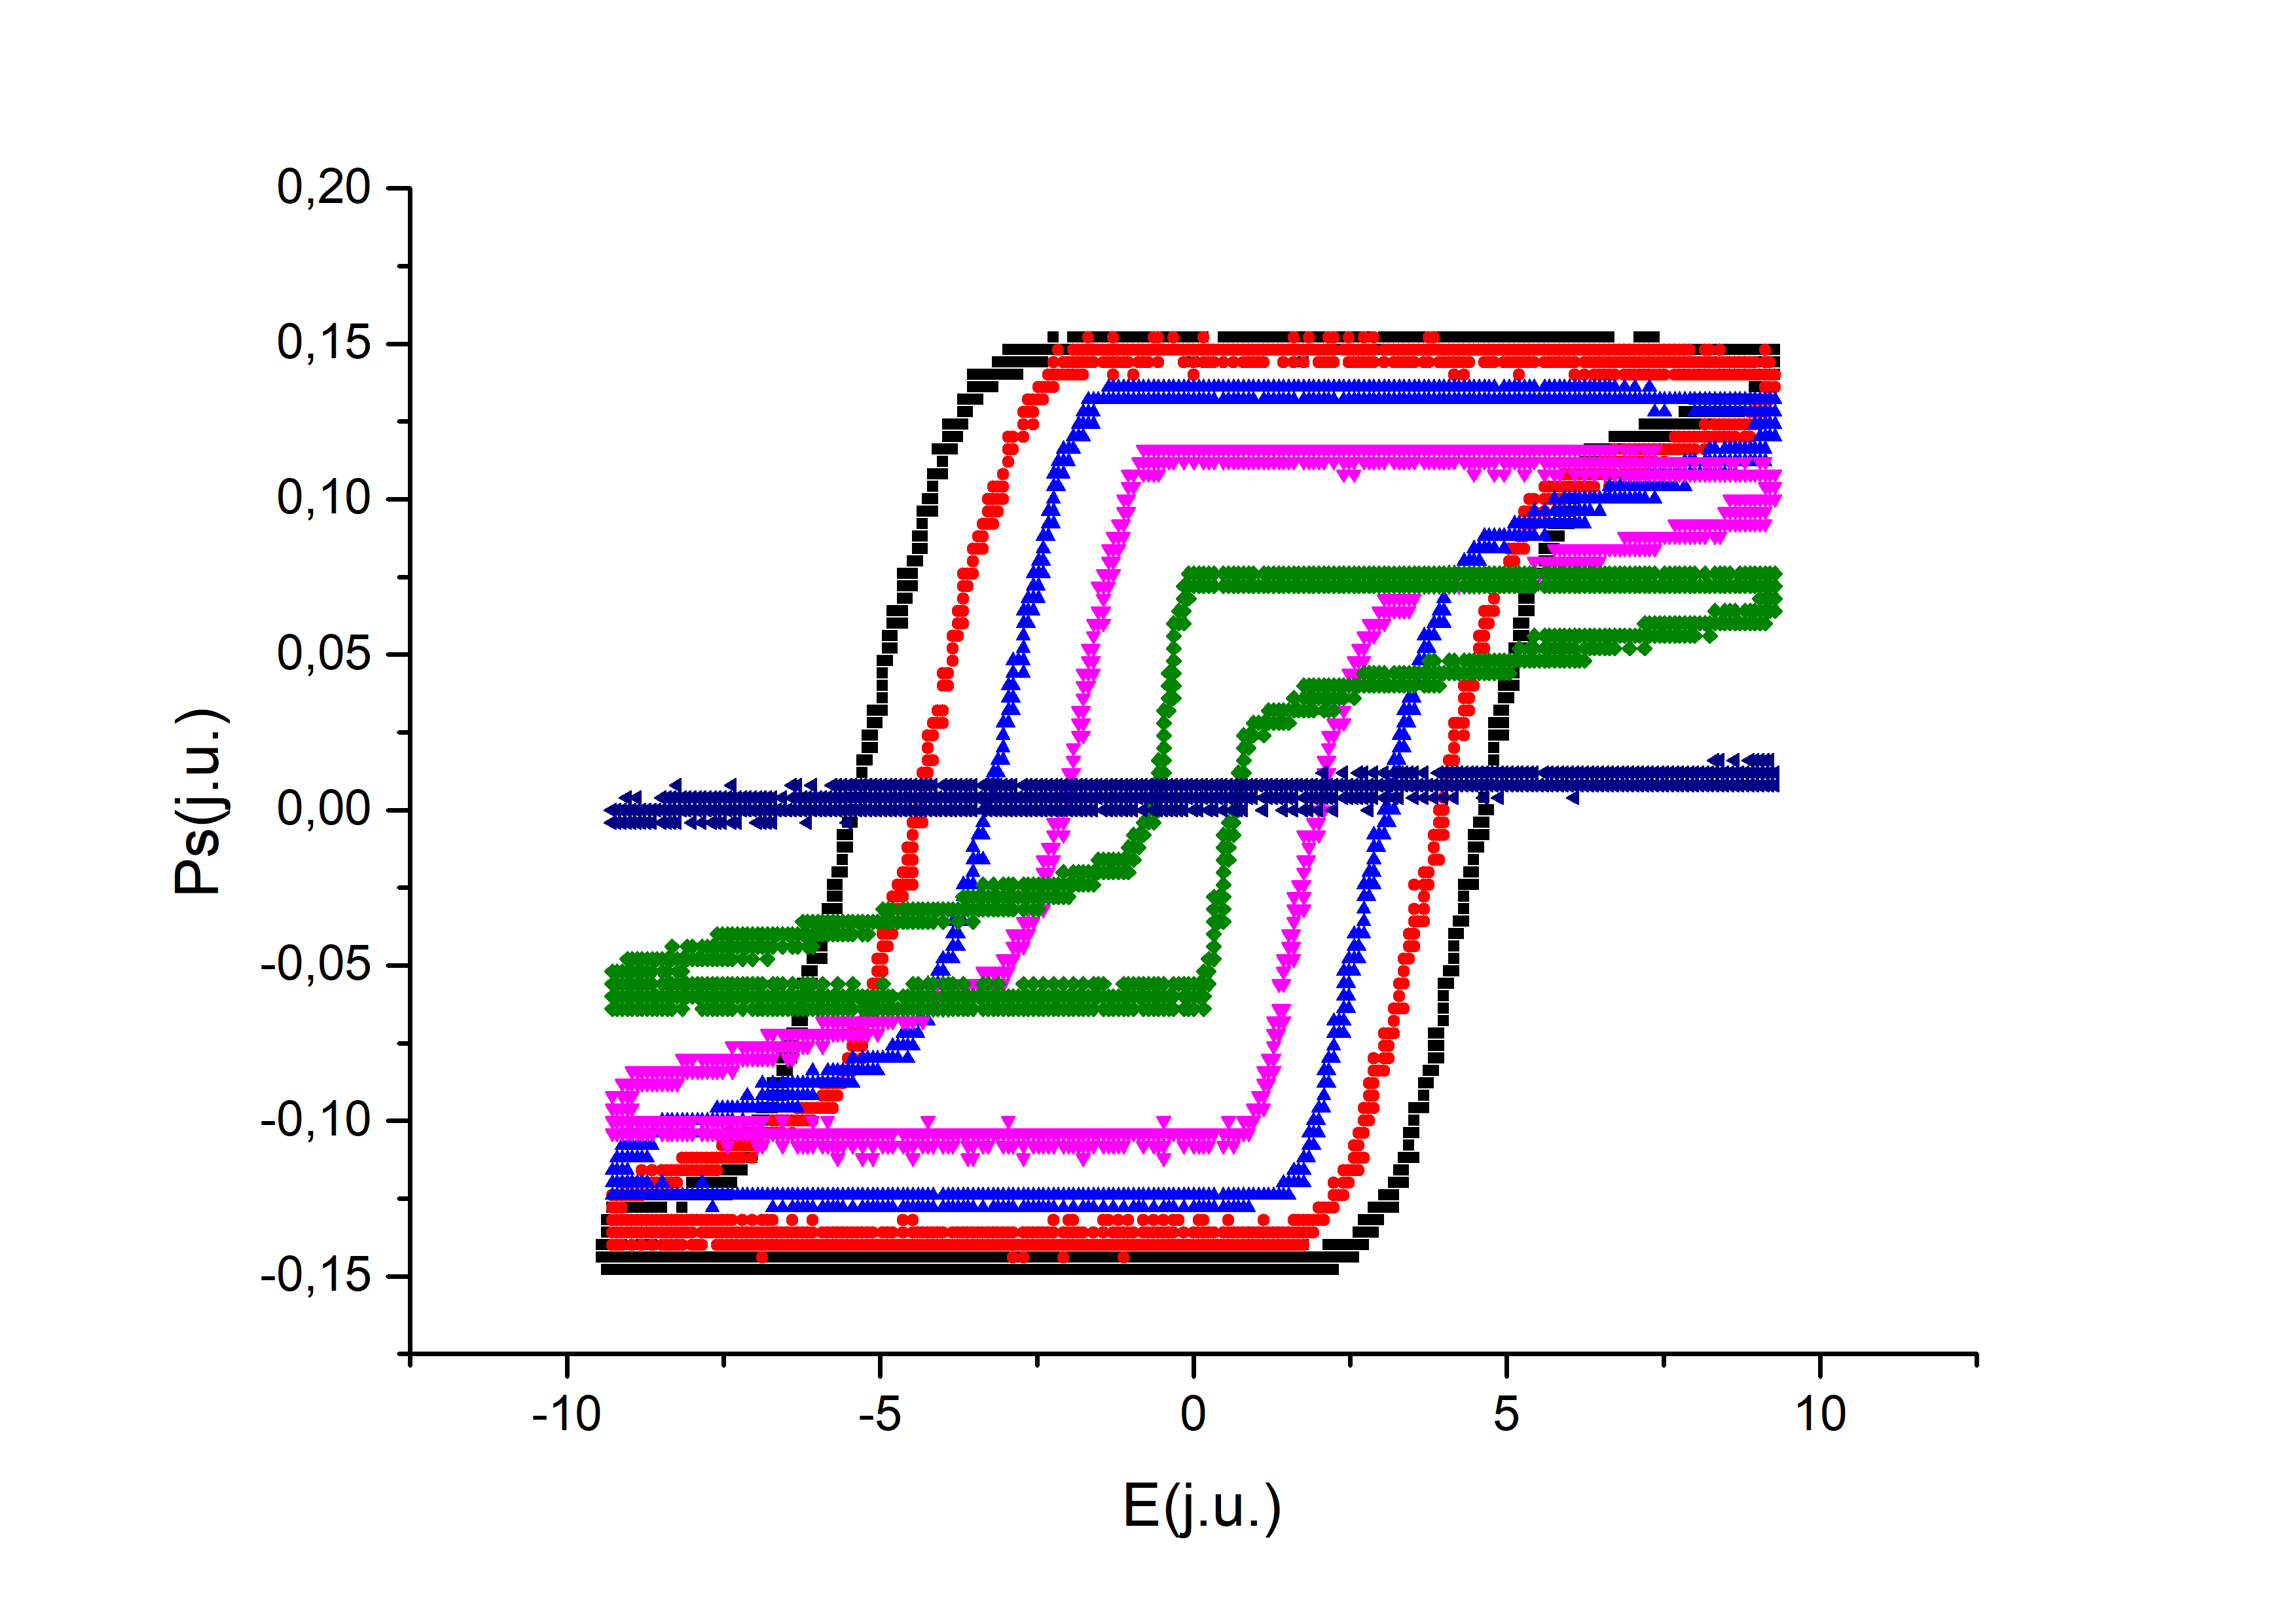
\includegraphics[width=0.8\linewidth]{Graph31.jpg}
	\caption{Przykładowe kształty pętli histerezy zaobserwowane podczas ogrzewania próbki, od temperatury pokojowej, aż do całkowitego zaniku pola koercji.}
	\label{fig:Graph31}
\end{figure}

Dla wszystkich z 27 otrzymanych pętli histerezy, zostały odczytane współrzędne przecięcia pętli z osiami układu współrzędnych oraz ekstrema pętli (wartości $X_{c}$,$Y_{c}$,$X_{max}$ i $Y_{max}$). Pętle nie były symetryczne względem początku układu współrzędnych, dlatego współrzędne przecięcia pętli z osiami musieliśmy uśrednić, w celu otrzymania wiarygodnego wyniku. Dzięki tym danym byliśmy w stanie wyznaczyć wartość przenikalności elektrycznej dla każdej pętli w stanie nasycenia, według wzoru:
\begin{equation}
\varepsilon_{max}=\dfrac{P_{max}}{\varepsilon_{0}\cdot E_{max}}
\end{equation}
gdzie $\varepsilon_{0}$ to wartość przenikalności elektrycznej w próżni, a $P_{max}$ obliczyliśmy za pomocą wzoru:
\begin{equation}
P_{max}=\dfrac{Y_{max}\cdot C_{0}}{S}
\end{equation}

Wartość $C_{0}$ jest wartością mostka DDP i w naszym modelu wynosiła ona $C_{0}=2\cdot10^{-6} F$. S w powyższym równaniu jest wartością pola powierzchni próbki kryształu i obliczyliśmy ją poprzez metodę histogramowego przetwarzania obrazu zdjęcia kryształu, zrobionego podczas pomiarów. Z analizy obrazy udało nam się wyliczyć wartość $S=4,00\cdot10^{-5} m^{2}$. Następnie dla każdej pętli policzyliśmy polaryzacje spontaniczną i pole koercji za pomocą wzorów:
\begin{equation}
P_{s}=\dfrac{Y_{c}\cdot C_{0}}{S}
\end{equation}
oraz 
\begin{equation}
E_{c}=\dfrac{X_{c}}{X_{max}}\cdot E_{max}
\end{equation}

Wykresy polaryzacji nasycenia $P_{max}$, polaryzacji spontanicznej $P_{s}$ oraz pola koercji $E_{c}$ w funkcji temperatury są pokazane na Rys.\ref{fig:Graph28}. i Rys.\ref{fig:Graph29}.

\begin{figure}[!h]
	\centering
	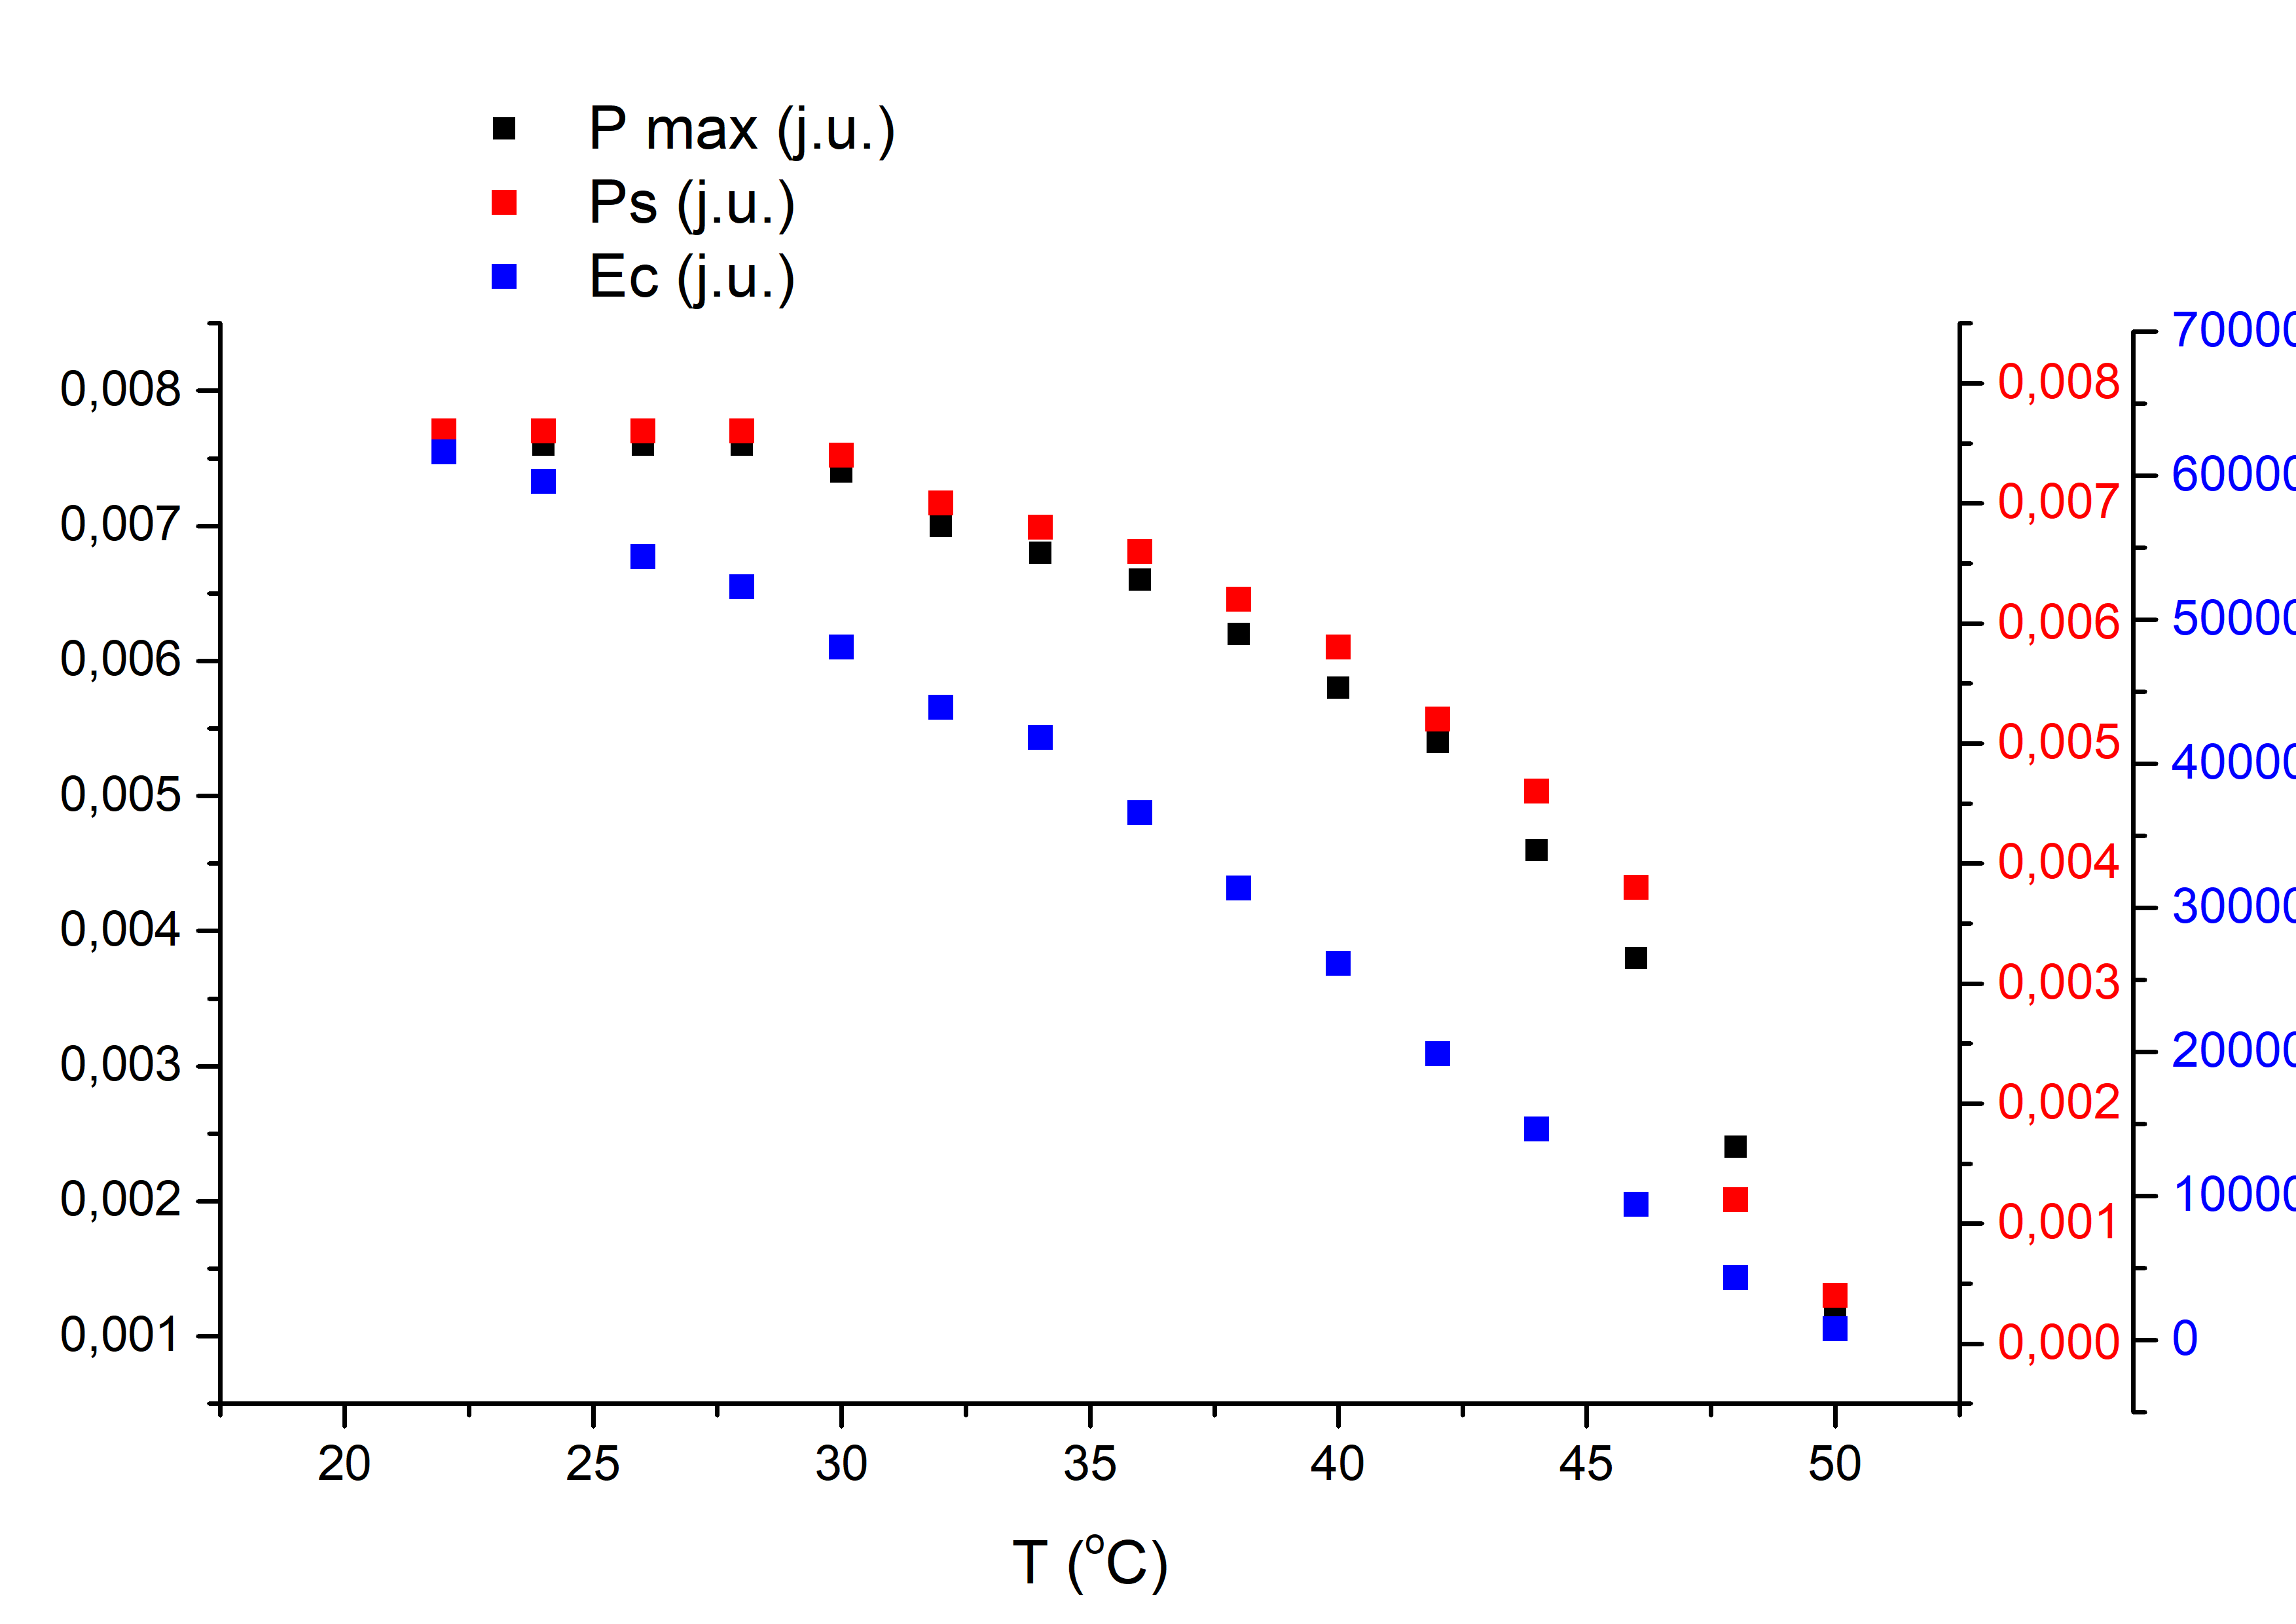
\includegraphics[width=0.8\linewidth]{Graph28.png}
	\caption{Wykresy polaryzacji nasycenia $P_{max}$, polaryzacji spontanicznej $P_{s}$ oraz pola koercji $E_{c}$ w funkcji temperatury dla ogrzewania próbki.}
	\label{fig:Graph28}
\end{figure}
\begin{figure}[!h]
	\centering
	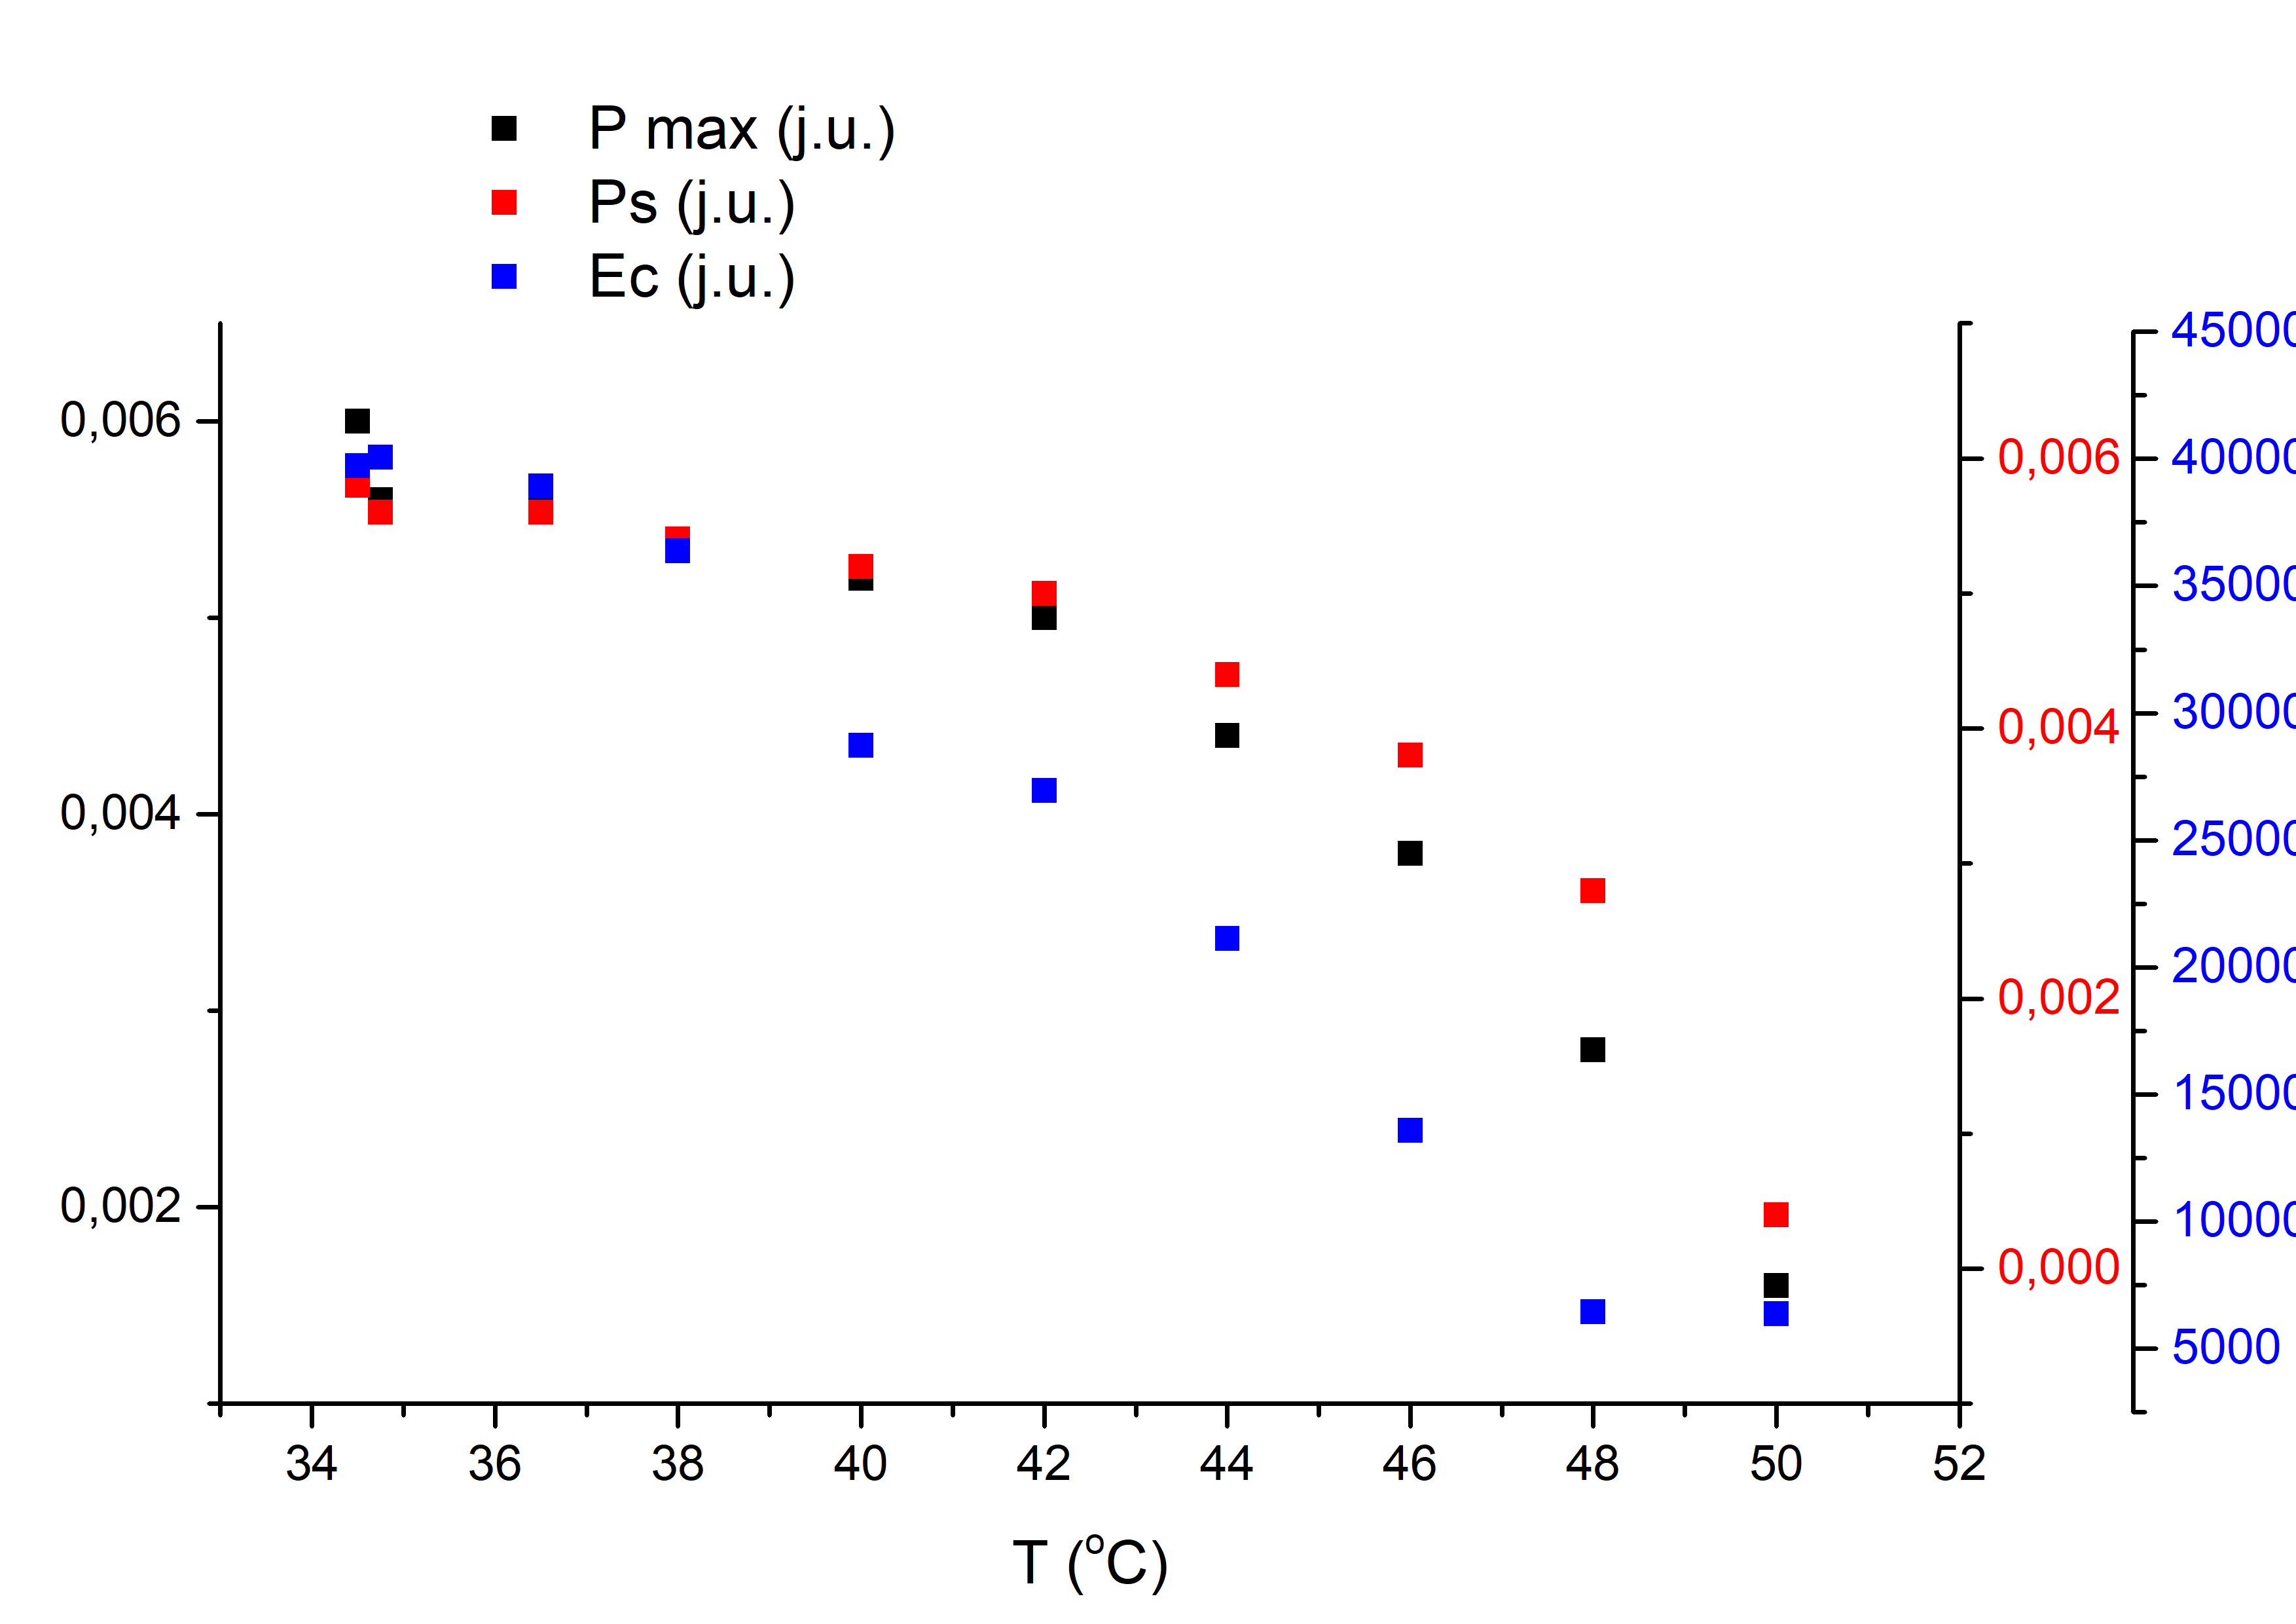
\includegraphics[width=0.8\linewidth]{Graph29.png}
	\caption{Wykresy polaryzacji nasycenia $P_{max}$, polaryzacji spontanicznej $P_{s}$ oraz pola koercji $E_{c}$ w funkcji temperatury dla ochładzania próbki.}
	\label{fig:Graph29}
\end{figure}

Na podstawie otrzymanych wyników jesteśmy w stanie narysować wykres zależności $P_{s}^{2}$ od temperatury (Rys.\ref{fig:Graph30}.). Dzięki niemu możemy oszacować że zakres temperatur dla którego $P_{s}^{2}$ jest liniową funkcją temperatury to zarówno dla ogrzewania jak i ochładzania 
\begin{equation}
T\in <42 , 50 > [^{o}C]
\end{equation}

\begin{figure}[!h]
	\centering
	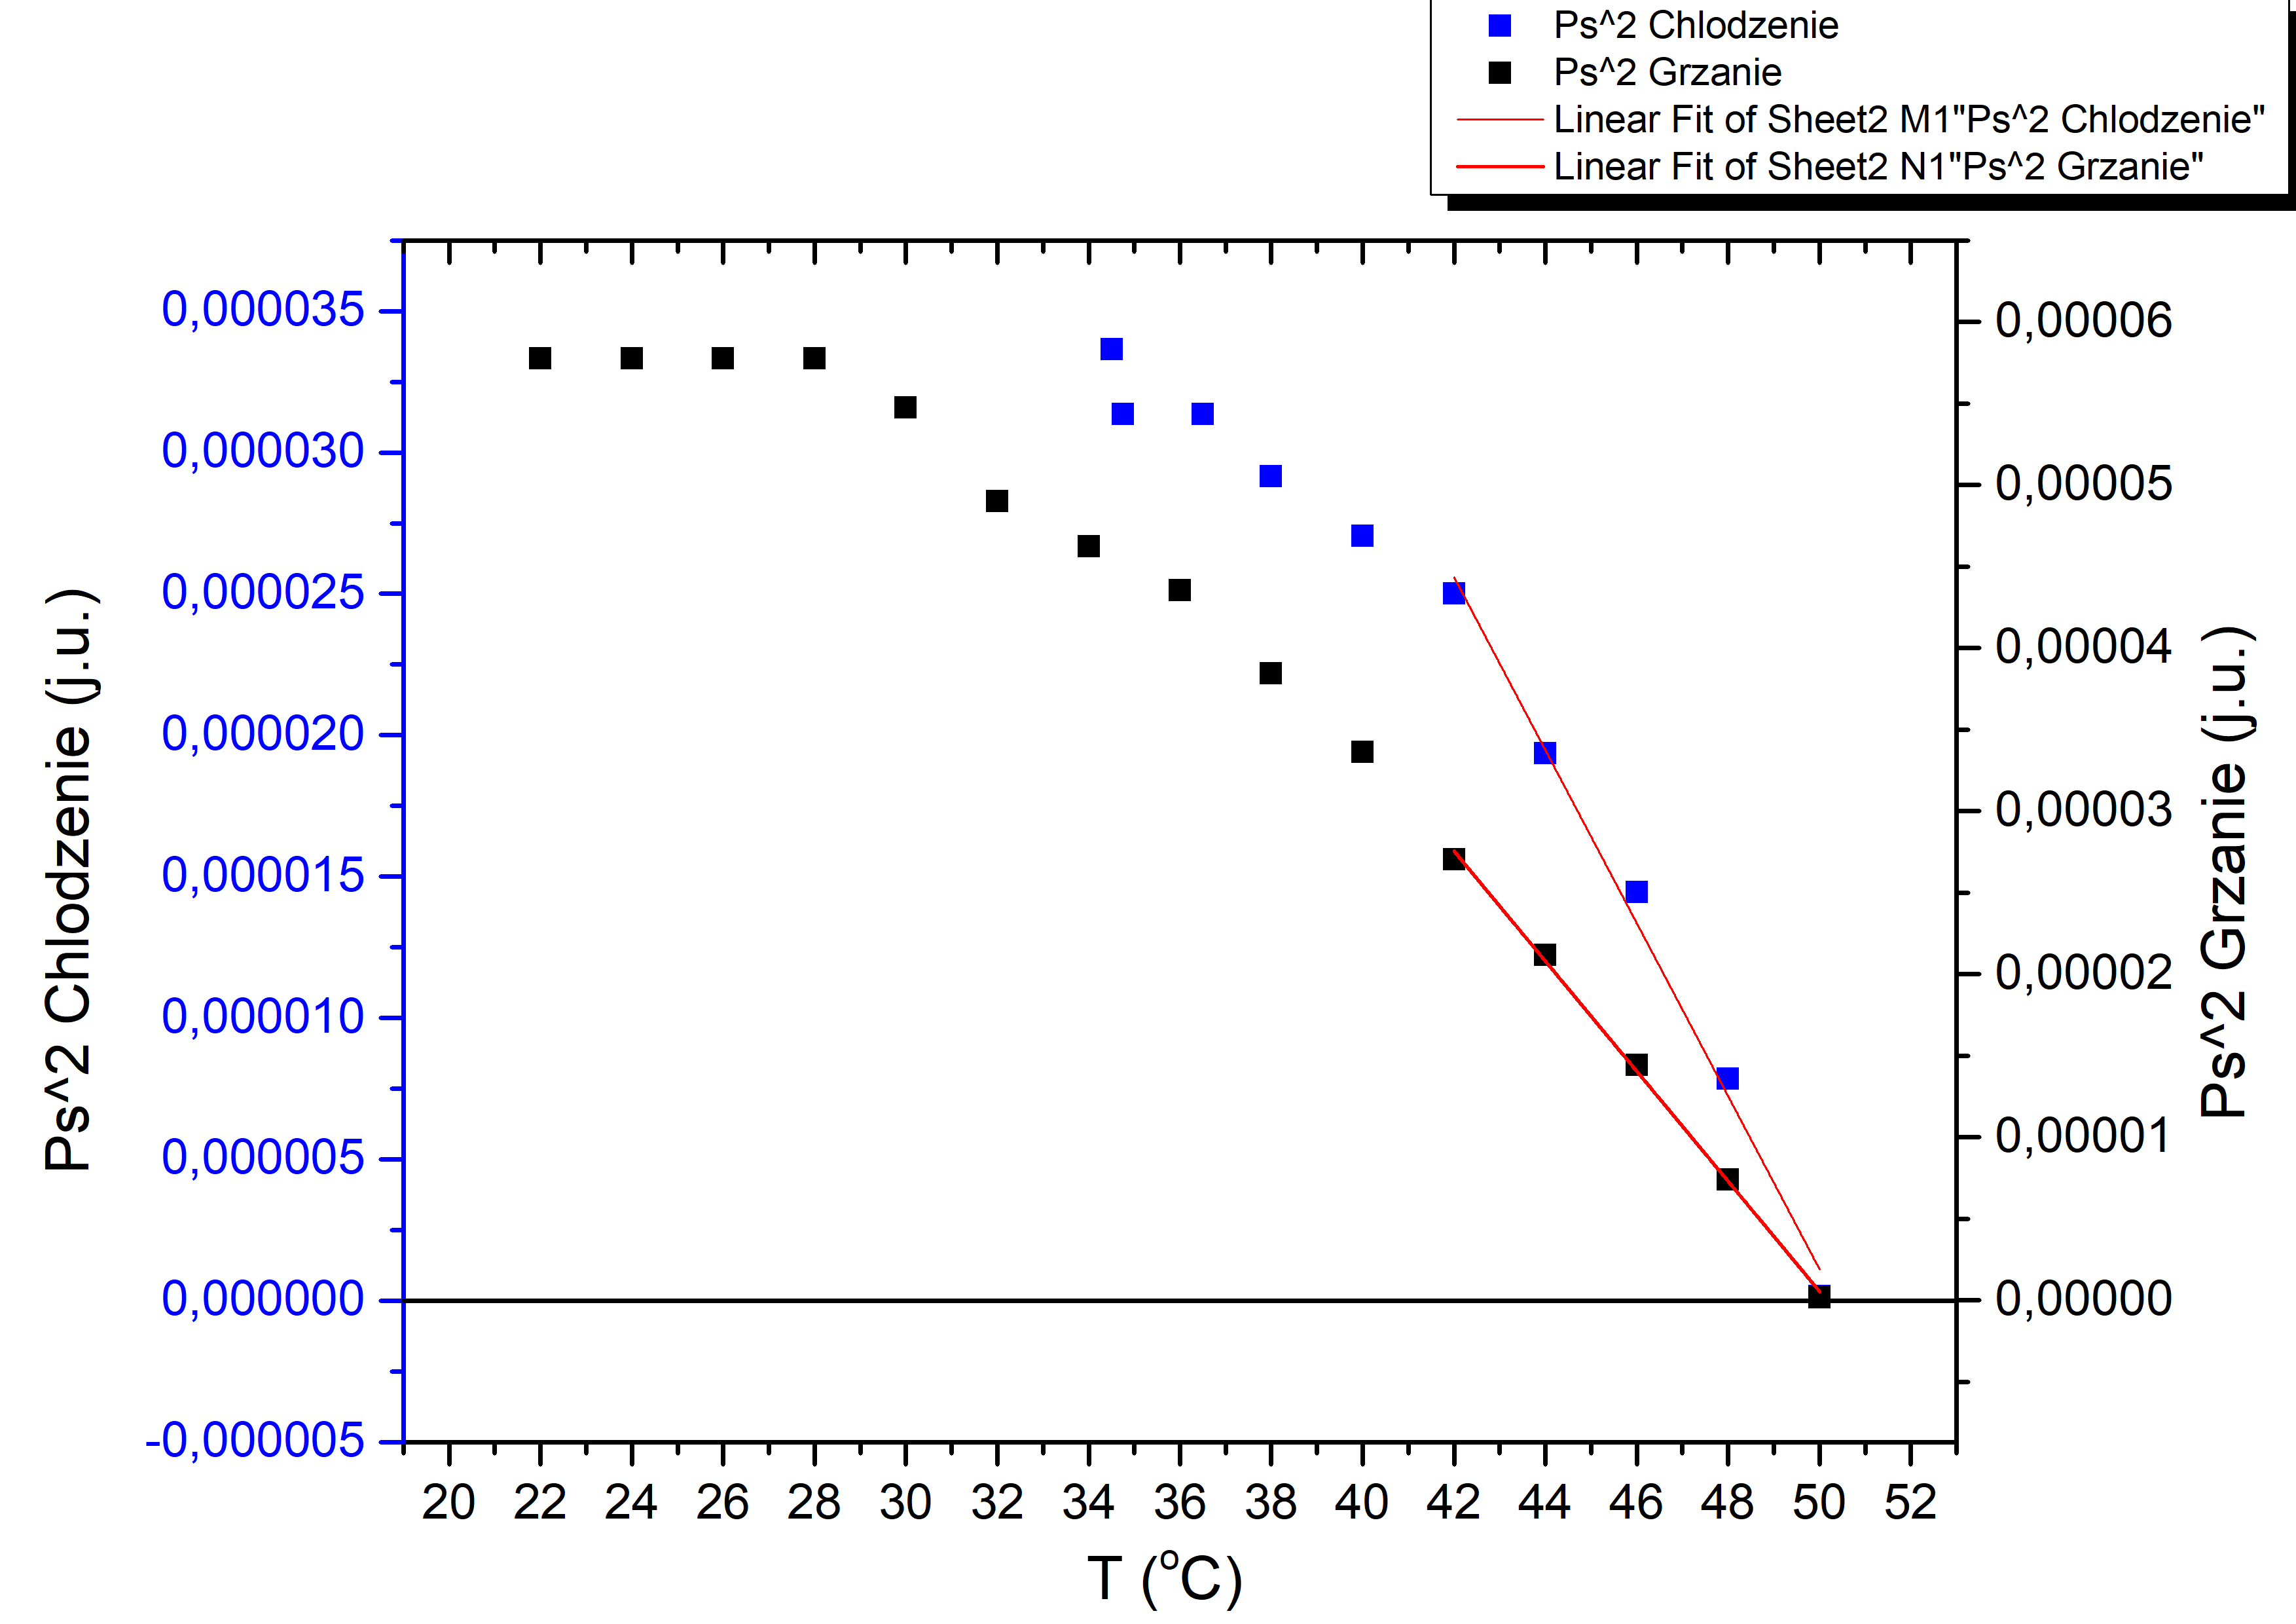
\includegraphics[width=0.8\linewidth]{Graph30.png}
	\caption{Wykres zależności $P_{s}^{2}$ od temperatury.}
	\label{fig:Graph30}
\end{figure}

\newpage
\subsection{Przenikalność elektryczna}
Żeby przystąpić do badania przenikalności elektrycznej kryształu TGS, musieliśmy najpierw stworzyć z niego kondensator, przy wykorzystaniu pasty srebrnej. Gdy już posiadaliśmy w pełni sprawny układ pomiarowy mogliśmy przejść do etapu pomiarów. W tym celu użyliśmy programu komputerowego o nazwie $Escort$ odczytującego bieżące parametry pojemności kondensatora dla danej temperatury. Próbkę badaliśmy dwa razy, pierwszy raz podgrzewaliśmy ją od temperatury pokojowej (około $16,5^{0}C$) do $100^{0}C$ w tempie $1^{0}C/min$. Po osiągnięciu tej temperatury wyciągnęliśmy próbkę z izolowanej termicznie komory, dzięki czemu zaczęła się ona ochładzać. Swobodne ochładzanie się próbki potrwało nieznacznie krócej niż jej ogrzanie, ale warto zaznaczyć że pomiar ten odbywał się tylko do temperatury $30^{0}C$. Uzyskane wyniki zaprezentowano na Rys.\ref{fig:wyk12}.

\begin{figure}[h!]
  \centering
  \begin{subfigure}[b]{0.49\linewidth}
    \includegraphics[width=\linewidth]{wyk1.png}
    \caption{}
  \end{subfigure}
  \begin{subfigure}[b]{0.49\linewidth}
    \includegraphics[width=\linewidth]{wyk2.png}
    \caption{}
  \end{subfigure}
  \caption{a)Wykres zależności pojemności kondensatora od temperatury podczas grzania. b)Wykres zależności pojemności kondensatora od temperatury podczas spontanicznego chłodzenia. Wykresy prezentują jedynie okolice temperatury Curie.}
  \label{fig:wyk12}
\end{figure}

Dzięki uzyskanym danym byliśmy w stanie obliczyć wartości przenikalności elektrycznej w badanym przedziale wg wzoru:
\begin{equation}
\varepsilon = \dfrac{C_{p}\cdot d}{S \cdot \varepsilon_{0}}
\end{equation}
gdzie $C_{p}$ jest odczytanym pomiarem pojemności kondensatora, d jest grubością kondensatora, S jest polem powierzchni kondensatora płaskiego, a $\varepsilon_{0}$ przenikalnością elektryczną w próżni. Otrzymane wyniki zaprezentowane są na Rys.\ref{fig:wyk3}.

\begin{figure}[!h]
	\centering
	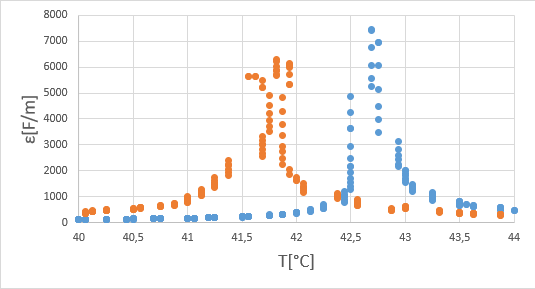
\includegraphics[width=0.7\linewidth]{wyk3.png}
	\caption{Wykres wartości przenikalności elektrycznej od temperatury próbki. Wykres pomarańczowy odpowiada chłodzeniu, a wykres niebieski odpowiada grzaniu. Wykres prezentuje jedynie okolice temperatury Curie. }
	\label{fig:wyk3}
\end{figure}

Następnie dzięki wykresom (Rys.\ref{fig:wyk45}.) $1/\varepsilon(T)$ byliśmy w stanie wyznaczyć wartość temperatury Curie, która dla grzania i chłodzenia wynosiła odpowiednio 
\begin{equation}
T_{C grz}=42,4523^{o}C
\end{equation}
oraz
\begin{equation}
T_{C chl}=41,5526^{o}C
\end{equation}

\begin{figure}[h!]
  \centering
  \begin{subfigure}[b]{0.49\linewidth}
    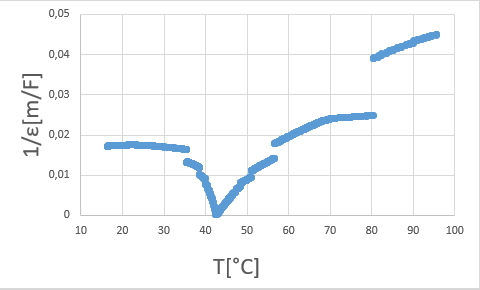
\includegraphics[width=\linewidth]{wyk4.png}
    \caption{}
  \end{subfigure}
  \begin{subfigure}[b]{0.49\linewidth}
    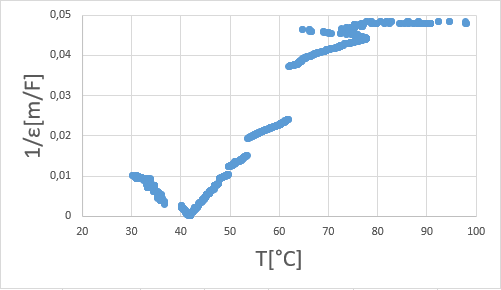
\includegraphics[width=\linewidth]{wyk5.png}
    \caption{}
  \end{subfigure}
  \caption{a)Wykres zależności pojemności odwrotności przenikalności elektrycznej od temperatury podczas grzania. b)Wykres zależności odwrotności przenikalności elektrycznej od temperatury podczas spontanicznego chłodzenia.}
  \label{fig:wyk45}
\end{figure}

Jak widać, wykresy $1/\varepsilon(T)$ są liniowe tylko dla pewnego przedziału zaraz po temperaturze Curie (Rys.\ref{fig:wyk67}.). Właśnie dla tego przedziału obowiązuje prawo Curie-Weissa i dla grzania zawiera się w przedziale :
\begin{equation}
T\in <42.4523 , 47.2500> [^{o}C]
\end{equation}
oraz dla chłodzenia :
\begin{equation}
T\in <41.5526 , 49.7500> [^{o}C]
\end{equation}

\begin{figure}[h!]
  \centering
  \begin{subfigure}[b]{0.49\linewidth}
    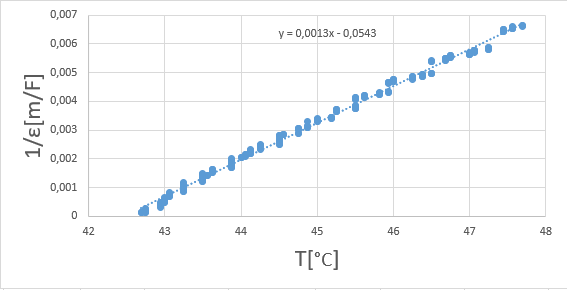
\includegraphics[width=\linewidth]{wyk6.png}
    \caption{}
  \end{subfigure}
  \begin{subfigure}[b]{0.49\linewidth}
    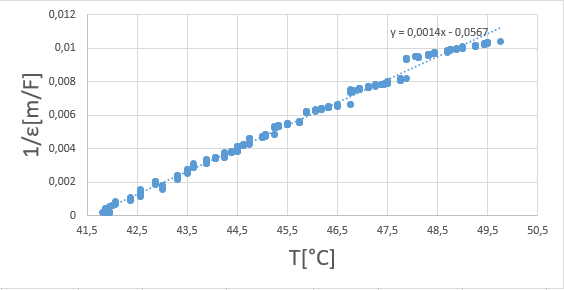
\includegraphics[width=\linewidth]{wyk7.png}
    \caption{}
  \end{subfigure}
  \caption{a)Wykres zależności pojemności odwrotności przenikalności elektrycznej od temperatury podczas grzania. b)Wykres zależności odwrotności przenikalności elektrycznej od temperatury podczas spontanicznego chłodzenia. Wykresy prezentują jedynie okolice temperatury Curie.}
\label{fig:wyk67}
\end{figure}

Dla fazy paraelektrycznej ($T-T_{c} > 0$ Rys.\ref{fig:wyk89}.), z odwrotności współczynnika kierunkowego prostej aproksymacji liniowej, można wyznaczyć stałą Curie-Weissa i dla grzania ma ona wartość:
\begin{equation}
C=1183,291 \pm 11,785 [K]
\end{equation}

oraz dla chłodzenia ma ona wartość:

\begin{equation}
C=912,9304 \pm 7,952 [K]
\end{equation}

\begin{figure}[h!]
  \centering
  \begin{subfigure}[b]{0.49\linewidth}
    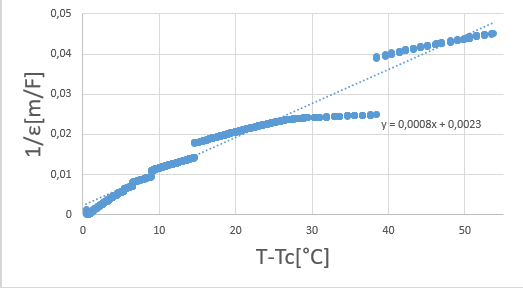
\includegraphics[width=\linewidth]{wyk9.png}
    \caption{}
  \end{subfigure}
  \begin{subfigure}[b]{0.49\linewidth}
    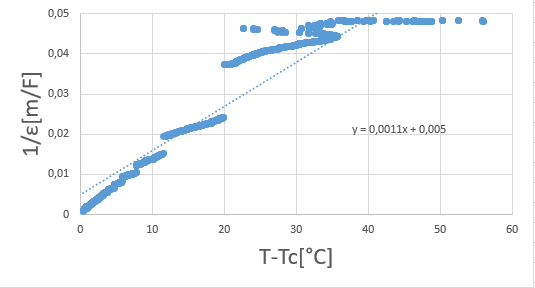
\includegraphics[width=\linewidth]{wyk8.png}
    \caption{}
  \end{subfigure}
  \caption{a)Wykres zależności pojemności odwrotności przenikalności elektrycznej od temperatury podczas grzania. b)Wykres zależności odwrotności przenikalności elektrycznej od temperatury podczas spontanicznego chłodzenia. Wykresy prezentują jedynie wartości powyżej temperatury Curie.}
\label{fig:wyk89}
\end{figure}

Ponadto otrzymane wyniki sprawdziliśmy pod kątem "prawa dwójki".Prawo to mówi, że stosunek przybliżeń liniowych wykresów $1/\varepsilon(T-T_{c})$ (Rys.\ref{fig:wyk1011}.) powinien mieć wartość przybliżoną do 2. Otrzymaliśmy wyniki: dla grzania $1,757$ oraz dla chłodzenia $1,407$.

\begin{figure}[h!]
  \centering
  \begin{subfigure}[b]{0.49\linewidth}
    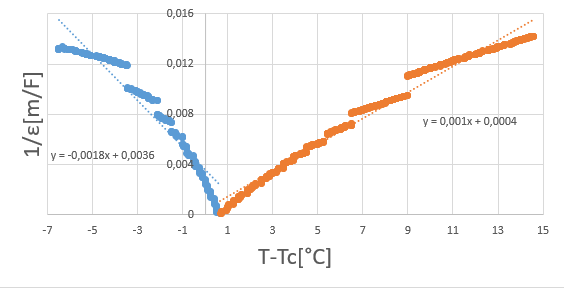
\includegraphics[width=\linewidth]{wyk10.png}
    \caption{}
  \end{subfigure}
  \begin{subfigure}[b]{0.49\linewidth}
    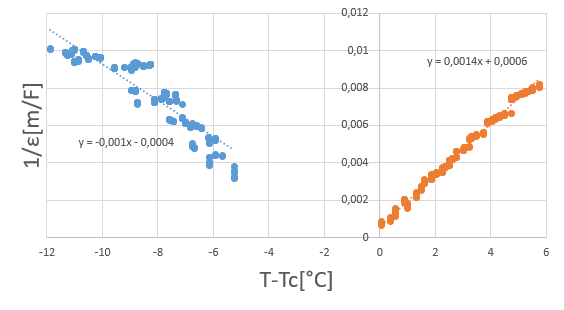
\includegraphics[width=\linewidth]{wyk11.png}
    \caption{}
  \end{subfigure}
  \caption{a)Wykres zależności pojemności odwrotności przenikalności elektrycznej od temperatury podczas grzania. b)Wykres zależności odwrotności przenikalności elektrycznej od temperatury podczas spontanicznego chłodzenia. Wykresy prezentują jedynie wartości powyżej temperatury Curie.}
\label{fig:wyk1011}
\end{figure}

\subsection{Dwójłomność spontaniczna}

Badanie zjawiska polaryzacji spontanicznej polegało na rejestrowaniu zmian natężenia światła przechodzącego przez cały układ, w zależności od temperatury układu. Laser He-Ne emitował światło laserowe o długości fali $\lambda=632nm$, które przechodziło przez dwa polaryzatory ustawione względem siebie pod kątem $90^{o}$. Kryształ TGS, który był ustawiony w kriostacie między polaryzatorem i analizatorem, wykazywał właściwości dwójłomne. Jego temperaturę zmienialiśmy od temperatury pokojowej, aż do temperatury około $100^{o}C$, a potem poddaliśmy próbkę swobodnemu chłodzeniu, także monitorując jej zachowanie. Wyniki jakie otrzymaliśmy zaprezentowane są na Rys.\ref{fig:wykD1}. i Rys.\ref{fig:wykD2}.

\begin{figure}[!h]
	\centering
	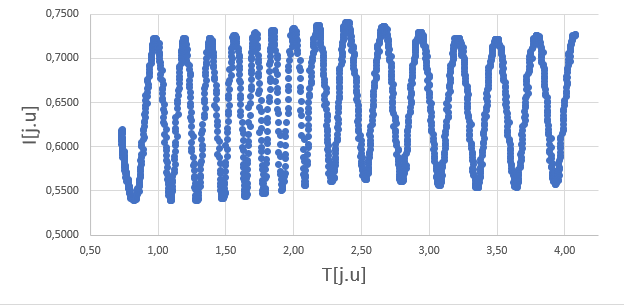
\includegraphics[width=0.7\linewidth]{wykD1.png}
	\caption{Wykres natężenia światła przechodzącego przez układ od temperatury kryształu, podczas ogrzewania próbki.}
	\label{fig:wykD1}
\end{figure}

\begin{figure}[!h]
	\centering
	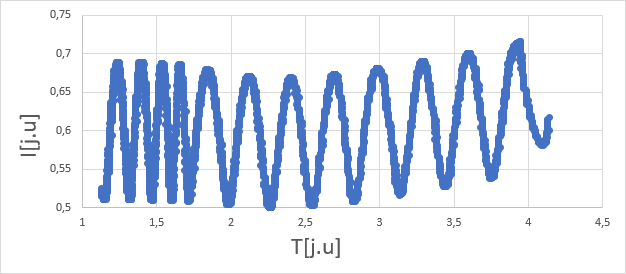
\includegraphics[width=0.7\linewidth]{wykD2.png}
	\caption{Wykres natężenia światła przechodzącego przez układ od temperatury kryształu, podczas swobodnego ochładzania próbki.}
	\label{fig:wykD2}
\end{figure}

Jak widać, proces chłodzenia trwał znacznie dłużej. Można to wywnioskować po zauważalnie większej liczbie punktów pomiarowych, w podobnym przedziale temperatur, co czyni drugi wykres bardziej 'ciągłym'. Kolejną rzeczą wartą zauważenia jest fakt, że natężenie zmienia się periodycznie. Jest to spowodowane różną drogą optyczną wiązek zwyczajnej i nadzwyczajnej, przez co po wyjściu z kryształu, gdy zaczynają interferować, są one w różnych fazach. Różnica między kolejnymi ekstremami jest przesunięciem o $\pi$, więc możemy narysować wykres zmian przesunięcia fazowego $\Gamma$ od temperatury $T$. Wykresy te pokazane są na Rys.\ref{fig:wykD3}. i Rys.\ref{fig:wykD4}.

\begin{figure}[!h]
	\centering
	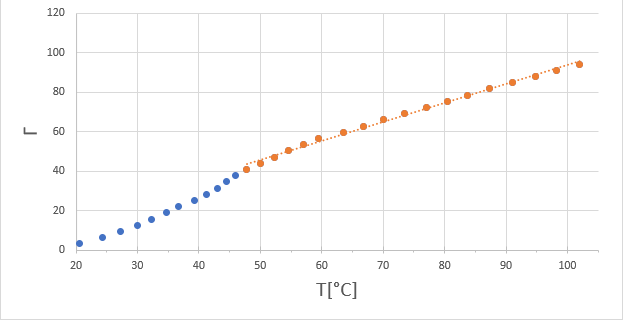
\includegraphics[width=0.7\linewidth]{wykD3.png}
	\caption{Wykres zmian przesunięcia fazowego od temperatury kryształu, podczas ogrzewania próbki.}
	\label{fig:wykD3}
\end{figure}

\begin{figure}[!h]
	\centering
	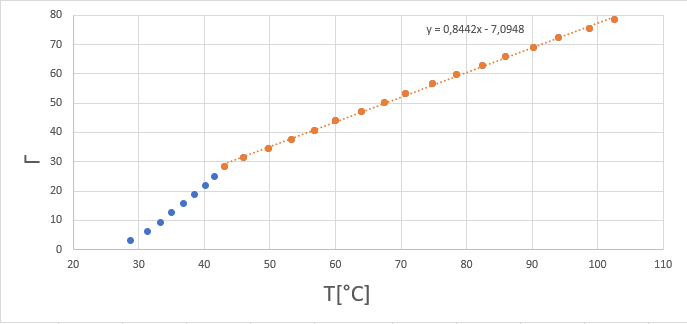
\includegraphics[width=0.7\linewidth]{wykD4.png}
	\caption{Wykres zmian przesunięcia fazowego od temperatury kryształu, podczas swobodnego ochładzania próbki.}
	\label{fig:wykD4}
\end{figure}

Jak widać na Rys.\ref{fig:wykD3}. i Rys.\ref{fig:wykD4}, w pewnym momencie wykres zaczyna przybierać kształt liniowy, lecz zanim się to stanie zależność zmian dwójłomności od temperatury wydaje się być funkcją nieliniową. Przemiana ma miejsce w Temperaturze Curie, po której funkcja staje się liniowa, a więc pochodna zmian dwójłomności równa jest 0. Wykres $\delta \Delta n(T)$ pokazany jest na Rys.\ref{fig:wykD5}. i Rys.\ref{fig:wykD6}.

\begin{figure}[!h]
	\centering
	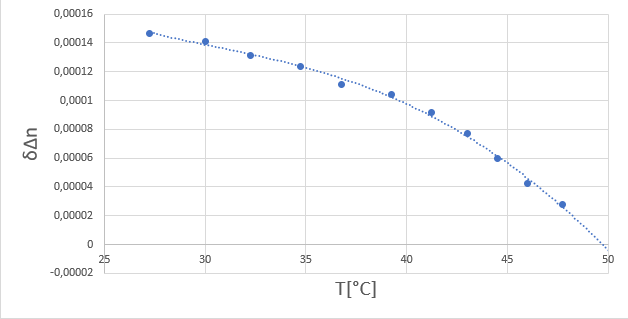
\includegraphics[width=0.7\linewidth]{wykD5.png}
	\caption{Wykres zmian miary dwójłomności od temperatury kryształu, podczas ogrzewania próbki.}
	\label{fig:wykD5}
\end{figure}

\begin{figure}[!h]
	\centering
	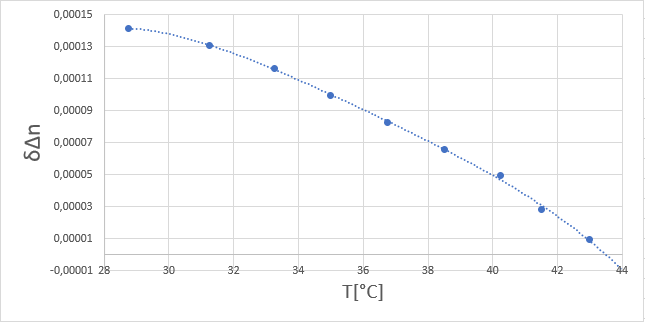
\includegraphics[width=0.7\linewidth]{wykD6.png}
	\caption{Wykres zmian miary dwójłomności od temperatury kryształu, podczas swobodnego ochładzania próbki.}
	\label{fig:wykD6}
\end{figure}

Z aproksymacji kwadratowej wykresów Rys.\ref{fig:wykD5}. i Rys.\ref{fig:wykD6}. można odczytać miejsce zerowe funkcji, czyli miejsce przemiany fazowej - wartość temperatury Curie. Wartości te to odpowiednio: dla ogrzewania próbki
\begin{equation}
T_{C grz}=49,8149^{o}C
\end{equation}
oraz dla spontanicznego chłodzenia próbki
\begin{equation}
T_{C chl}=43,5187^{o}C
\end{equation}

\section{Dyskusja wyników}
Wnioskując na podstawie uzyskanych wyników można uznać, że badania zostały przeprowadzone poprawnie, a wyniki są zbliżone do tablicowych \cite{antoniewicz}. Podsumowując, temperatury Curie wyznaczone dla kryształu podczas badań to:\\
- dla zjawiska polaryzacji spontanicznej wartość $50^{o}C$ i była to najmniej dokładna metoda do otrzymania tej wartości.\\
- dla zjawiska przenikalności elektrycznej były to wartości odpowiednio dla ogrzewania i chłodzenia próbki $T_{C grz}=42,4523^{o}C$ oraz $T_{C chl}=41,5526^{o}C$. Było to doświadczenie dające najbardziej spójny i najlepszy jakościowo wynik temperatury Curie.\\
- dla zjawiska dwójłomności spontanicznej była to wartości odpowiednio dla ogrzewania i chłodzenia próbki $T_{C grz}=49,8149^{o}C$ oraz $T_{C chl}=43,5187^{o}C$. Było to badanie dające dobry jakościowo wynik, niestety z dużą rozbieżnością dla ogrzewania materiału i ochładzania go.\\
Warto wziąć pod uwagę fakt, że chłodzenie spontaniczne odbywało się w mało kontrolowany sposób, z powodu dużego ruchu w sali pomiarowej, otwierania drzwi i okien, które mogły mieć wpływ na tempo ochładzania się próbek, a na pewno powodowało, że ten proces był niejednostajny i chaotyczny.
Ewie już działa Latex, teraz ogarnijmy gita pls

\begin{thebibliography}{99}
	\bibitem{krajewski} Krajewski T. \textit{Zagadnienia fizyki dielektryków}, Wydawnictwa Komunikacji i Łączności, Warszawa 1970 
	\bibitem{histereza}Dragan Damjanovic \textit{Hysteresis in Piezoelectric
and Ferroelectric Materials}, The Science of Hysteresis, Volume 3; I. Mayergoyz and G.Bertotti (Eds.); Elsevier (2005)
	\bibitem{malus} Jurgen R. Meyer-Arendt: \textit{Wstęp do optyki.} Wyd. 1. Warszawa: Państwowe Wydawnictwo Naukowe, 1977.
	\bibitem{dwoj} Richard Phillips Feynman, Robert B. Leighton, Matthew Sands: \textit{Feynmana wykłady z fizyki.} T. 1. Cz. 2. Wydawnictwo Naukowe PWN.
	\bibitem{antoniewicz} Jerzy Antoniewicz \textit{Własności dielektrykow, Tablice i wykresy}, Wydawnictwa Naukowo-Techniczne, Warszawa 1971
\end{thebibliography}
\end{document}
